% ============================================================================
% AIDER — AI-Driven Energy Research
% Paper Template v1.0
%
% INSTRUCTIONS FOR AUTHORS:
%   - Fill in your title, authors, affiliations, and abstract below
%   - Write your paper in the sections provided
%   - Do NOT modify the header block (lines marked "EDITORIAL USE ONLY")
%   - The editorial header will be populated automatically upon acceptance
%
% INSTRUCTIONS FOR EDITORS (post-acceptance):
%   - Set \acceptedtrue (line ~65)
%   - Fill in \aiderdoi, \aidervolume, \aiderissue, \aideryear, \aiderpages
%   - Fill in \editorname, \reviewernames, \submitteddate, \accepteddate, \publisheddate
%   - Replace the text logo with \includegraphics when logo file is ready
% ============================================================================

\documentclass[11pt, a4paper]{article}

% --- Core packages ---
\usepackage[utf8]{inputenc}
\usepackage[T1]{fontenc}
\usepackage{lmodern}
\usepackage[top=2.5cm, bottom=2.5cm, left=2.5cm, right=2.5cm]{geometry}
\usepackage{amsmath, amssymb}
\usepackage{graphicx}
\usepackage[dvipsnames]{xcolor}
\usepackage{fancyhdr}
\usepackage{titlesec}
\usepackage{booktabs}
\usepackage{caption}
\usepackage{ifthen}
\usepackage{indentfirst}
\usepackage{graphicx}
\usepackage{subcaption}
\usepackage[percent]{overpic}
\usepackage{xcolor}
\usepackage[backend=biber,
            style=numeric,
            sorting=none,
            doi=true,
            url=false]{biblatex}
\usepackage[colorlinks=true,
            linkcolor=blue,
            citecolor=blue,
            urlcolor=blue]{hyperref}
\addbibresource{references.bib}

\DeclareFieldFormat{doi}{%
  \par\noindent\href{https://doi.org/#1}{doi:#1}
}

% --- Colours ---
\definecolor{aiderblue}{HTML}{2563EB}
\definecolor{aiderdark}{HTML}{0A0F1A}
\definecolor{aidergrey}{HTML}{6B7280}
\definecolor{aiderlight}{HTML}{F3F4F6}
\definecolor{aidergreen}{HTML}{059669}

% --- Hyperref setup ---
\hypersetup{
    colorlinks=true,
    linkcolor=aiderblue,
    citecolor=aiderblue,
    urlcolor=aiderblue,
    pdfborder={0 0 0}
}

\captionsetup[subfigure]{labelformat=empty}

% ============================================================================
% EDITORIAL METADATA — filled upon acceptance (do not modify as author)
% ============================================================================

% Set to true when paper is accepted and published
\newif\ifaccepted
\acceptedfalse  % ← Editor sets to \acceptedtrue

% Publication metadata (EDITORIAL USE ONLY)
\newcommand{\aiderdoi}{10.5281/zenodo.XXXXXXX}
\newcommand{\aidervolume}{1}
\newcommand{\aiderissue}{1}
\newcommand{\aideryear}{2026}
\newcommand{\aiderpages}{1--XX}
\newcommand{\editorname}{@editor-github}
\newcommand{\reviewernames}{@reviewer1, @reviewer2}
\newcommand{\submitteddate}{YYYY-MM-DD}
\newcommand{\accepteddate}{YYYY-MM-DD}
\newcommand{\publisheddate}{YYYY-MM-DD}
\newcommand{\repourl}{https://github.com/author/repo}
\newcommand{\reviewurl}{https://github.com/ai-driven-energy-research/submissions/issues/XX}
\renewcommand{\thesubfigure}{\Alph{subfigure}}

% ============================================================================
% AUTHOR METADATA — fill these in
% ============================================================================

\newcommand{\papertitle}{A Data-Driven Design Strategy for Next-Generation \\Lithium Batteries: Feature-Guided Development of  \\Diluent for High-Performance Electrolytes}
\newcommand{\paperauthors}{Jingda Wu$^{1}$}
\newcommand{\paperaffiliations}{%
    $^{1}$Graduate School of Energy Science, Kyoto University, Kyoto, Japan.\\
}
\newcommand{\paperemail}{wu.jingda.43k@st.kyoto-u.ac.jp}
\newcommand{\paperkeywords}{Lithium-ion batteries, High-concentration electrolytes, Fluorinated diluents, Feature importance analysis, SHAP analysis}

% ============================================================================
% HEADER / FOOTER (subsequent pages)
% ============================================================================

\pagestyle{fancy}
\fancyhf{}
\renewcommand{\headrulewidth}{0.4pt}
\renewcommand{\footrulewidth}{0.4pt}

\lhead{\fontfamily{phv}\selectfont\footnotesize\color{aidergrey}%
    \textbf{AIDER} \textbar\ AI-Driven Energy Research}
\rhead{\fontfamily{phv}\selectfont\footnotesize\color{aidergrey}%
    \ifaccepted Vol.~\aidervolume, No.~\aiderissue~(\aideryear)%
    \else Preprint\fi}

\lfoot{\fontfamily{phv}\selectfont\scriptsize\color{aidergrey}%
    \ifaccepted \href{https://doi.org/\aiderdoi}{https://doi.org/\aiderdoi}%
    \else \textit{Under review at AI-Driven Energy Research}\fi}
\rfoot{\fontfamily{phv}\selectfont\scriptsize\color{aidergrey}\thepage}

% --- First page: no header rule, custom footer ---
\fancypagestyle{plain}{%
    \fancyhf{}
    \renewcommand{\headrulewidth}{0pt}
    \renewcommand{\footrulewidth}{0.4pt}
    \lfoot{\fontfamily{phv}\selectfont\scriptsize\color{aidergrey}%
        \ifaccepted \href{https://doi.org/\aiderdoi}{https://doi.org/\aiderdoi}%
        \else \textit{Under review at AI-Driven Energy Research}\fi}
    \rfoot{\fontfamily{phv}\selectfont\scriptsize\color{aidergrey}\thepage}
}

% --- Section styling ---
\titleformat{\section}
    {\fontfamily{phv}\selectfont\Large\bfseries\color{aiderdark}}
    {\thesection}{0.8em}{}
\titleformat{\subsection}
    {\fontfamily{phv}\selectfont\large\bfseries\color{aiderdark}}
    {\thesubsection}{0.8em}{}
\titleformat{\subsubsection}
    {\fontfamily{phv}\selectfont\normalsize\bfseries\color{aiderdark}}
    {\thesubsubsection}{0.8em}{}

% --- Caption styling ---
\captionsetup{
    font={small, sf},
    labelfont={bf, color=aiderdark},
    margin=1em
}

% ============================================================================
% AIDER BANNER COMMAND
% ============================================================================

\newcommand{\aiderbanner}{%
    % --- Dark banner ---
    \noindent\colorbox{aiderdark}{%
        \parbox{\dimexpr\textwidth-2\fboxsep\relax}{%
            \vspace{8pt}%
            \hspace{6pt}%
            % TODO: Replace with \includegraphics[height=1cm]{aider-logo.pdf}
            {\fontfamily{phv}\selectfont\bfseries\color{white}\Large AIDER}%
            \hspace{8pt}%
            {\fontfamily{phv}\selectfont\color{white!70}\small AI-Driven Energy Research}%
            \hfill%
            {\fontfamily{phv}\selectfont\color{aidergreen}\footnotesize\bfseries Diamond Open Access}%
            \hspace{6pt}%
            \vspace{8pt}%
        }%
    }%

    % --- Blue accent line ---
    \noindent\colorbox{aiderblue}{%
        \parbox{\dimexpr\textwidth-2\fboxsep\relax}{\vspace{1.5pt}}%
    }%

    \vspace{10pt}%

    % --- Metadata block ---
    \ifaccepted
        {\fontfamily{phv}\selectfont\scriptsize\color{aidergrey}%
        \noindent
        \begin{tabular}{@{}l@{\hspace{1.2em}}l@{\hspace{1.2em}}l@{}}
            \textbf{DOI:} \href{https://doi.org/\aiderdoi}{\aiderdoi}
            & \textbf{Volume:} \aidervolume(\aiderissue), pp.~\aiderpages
            & \textbf{Published:} \publisheddate \\[4pt]
            \textbf{Editor:} \editorname
            & \textbf{Reviewers:} \reviewernames
            & \textbf{Submitted:} \submitteddate \\[4pt]
            \textbf{Repository:} \href{\repourl}{GitHub}
            & \textbf{Review:} \href{\reviewurl}{Submission Issue}
            & \textbf{Accepted:} \accepteddate \\
        \end{tabular}%
        }%
    \else
        {\fontfamily{phv}\selectfont\scriptsize\color{aidergrey}%
        \noindent
        \begin{tabular}{@{}l@{\hspace{2em}}l@{\hspace{2em}}l@{}}
            \textbf{DOI:} \textit{assigned upon acceptance}
            & \textbf{Volume / Issue:} \textit{assigned upon acceptance}
            & \textbf{Status:} \textit{Preprint / Under Review} \\[4pt]
            \textbf{Editor:} \textit{assigned upon submission}
            & \textbf{Reviewers:} \textit{assigned upon submission}
            & \textbf{License:} CC-BY 4.0 \\
        \end{tabular}%
        }%
    \fi

    \vspace{4pt}%
    \noindent\rule{\textwidth}{0.4pt}%
}

% ============================================================================
% DOCUMENT
% ============================================================================

\begin{document}
\thispagestyle{plain}

% --- AIDER Banner ---
\aiderbanner

\vspace{0.6cm}

% --- Title ---
{\fontfamily{phv}\selectfont\LARGE\bfseries\color{aiderdark}
\papertitle\par}

\vspace{0.5cm}

% --- Authors ---
{\fontfamily{phv}\selectfont\normalsize\color{aidergrey}
\paperauthors\par}

\vspace{0.25cm}

% --- Affiliations ---
{\fontfamily{phv}\selectfont\small\color{aidergrey}
\paperaffiliations\par}

\vspace{0.15cm}

% --- Contact ---
{\fontfamily{phv}\selectfont\small
\href{mailto:\paperemail}{\paperemail}\par}

\vspace{0.6cm}

% --- Abstract ---
\noindent\rule{\textwidth}{0.4pt}
\vspace{0.2cm}
{\fontfamily{phv}\selectfont\footnotesize\bfseries\color{aiderdark} ABSTRACT}
\vspace{0.15cm}

\noindent
{\small The development of high-performance electrolytes remains a critical bottleneck in advancing lithium-ion battery technology, with high-concentration electrolytes (HCEs) offering enhanced electrochemical stability but suffering from poor ionic conductivity. Here, a data-driven framework is established to integrate experimental measurements, quantum chemical calculations, and machine learning, facilitating the design of fluorinated diluents that optimize ionic conductivity in localized HCE systems. By systematically investigating four fluorinated benzene derivatives in 3 M LiFSI-DME electrolyte, a trade-off between viscosity reduction and ion dilution that governs conductivity enhancement is revealed. Through comparative evaluation of polynomial fitting and machine learning regression methods, this study shows that model complexity should match the dataset—a third-order polynomial achieved high predictive accuracy, while more complex algorithms showed no advantage, providing practical guidance for small datasets. Shapley additive explanations (SHAP) are employed to identify frontier orbital energies and dielectric constant as the dominant molecular descriptors controlling ionic conductivity, leading to several design principles: optimal diluents require high HOMO/LUMO energies to minimize lithium coordination, moderate dielectric constants for ion dissociation, and low molecular weights for enhanced mobility.
This work is not limited to LiFSI-DME electrolyte system and establishes a generalizable strategy that combines interpretable machine learning with mechanistic insight to accelerate materials discovery. By demonstrating how limited experimental data can be transformed into predictive design rules through AI-assisted analysis, this work provides a useful reference for future battery development that helps move from trial-and-error experimentation toward more rational, computation-guided materials design. This approach may help accelerate the optimization of complex electrochemical systems and advance the broader field of AI-driven energy materials research.}

\vspace{0.2cm}
\noindent\rule{\textwidth}{0.4pt}

\vspace{0.2cm}
{\fontfamily{phv}\selectfont\footnotesize\color{aidergrey}
\textbf{Keywords:} \paperkeywords}

\vspace{0.6cm}

% ============================================================================
% PAPER BODY — write your paper below
% ============================================================================

\clearpage

\section{Introduction}

{Lithium-ion batteries (LIBs) have become an important technology in energy applications, supporting applications ranging from portable electronics to electric vehicles and large-scale energy storage systems\cite{ref.1}. Advantages such as high energy density, long cycle life, and relatively mature manufacturing processes have made LIBs a key component in the transition toward carbon-neutral energy systems. In response to the demand for high performance and improved safety of LIBs, the development of advanced electrolyte systems has become an important research topic\cite{ref.2}. Among the electrolytes studied, high-concentration electrolytes (HCEs), such as 3 M LiFSI dissolved in dimethoxyethane (DME)\cite{ref.3}, have been widely studied. Compared with conventional dilute electrolytes, HCEs exhibit enhanced electrochemical stability, improved compatibility with high-voltage cathodes, and the ability to facilitate the formation of solid electrolyte interphase (SEI)\cite{ref.4}. These advantages derive from their unique solvation structure, in which a larger fraction of solvent molecules coordinate with lithium ions\cite{ref.5}. However, HCEs still face significant challenges that limit their practical application, such as comparatively high viscosity\cite{ref.6} and low ionic conductivity\cite{ref.7}, which hinder their rate performance. In addition, sluggish ion transport promotes lithium plating during the charging process, raising safety concerns and degrading battery lifespan\cite{ref.7}.

To address these limitations, an effective strategy involving the introduction of diluents into HCEs has been widely explored. Diluents are typically non-coordinating or weakly coordinating solvents that can reduce the viscosity of the electrolyte without significantly disrupting the localized high-concentration solvation structure\cite{ref.8}. By lowering the viscosity, diluents enhance the ionic conductivity of the electrolytes and ideally preserve the favorable SEI formation between HCEs and electrodes\cite{ref.8}. Among various diluents, fluorinated benzene derivatives, such as fluorobenzene (FBn)\cite{ref.8}, 1,2-difluorobenzene (dFBn)\cite{ref.9}, 1,3,5-trifluorobenzene (tFBn)\cite{ref.10}, and hexafluorobenzene (hFBn)\cite{ref.11}, have been reported as promising candidates owing to their low donor numbers, electrochemical stability, and compatibility with lithium salts. Their fluorinated functional groups also contribute to the formation of stable SEIs, which further improves the cycling performance of LIBs employing these electrolyte systems\cite{ref.10}. These characteristics suggest that they are promising of fluorinated benzene derivatives as ideal additives for next-generation HCEs in LIBs.

Despite these advantages, several questions remain unanswered in the study of fluorinated benzene derivatives. For example, previous studies have not systematically investigated the optimal concentration of each diluent for achieving maximum ionic conductivity\cite{ref.8}-\cite{ref.11}. As a result, the most effective volume fraction for each diluent system remains unclear, limiting performance optimization. In addition, the fundamental mechanisms by which multiple diluent features enhance ionic conductivity have not been systematically analyzed. The relationship between the molecular features of diluents and the electrochemical performance of HCEs remains ambiguous. Fluorinated benzene derivatives differ in multiple physical and chemical properties, such as the position and number of fluorine functional groups, polarity, and molecular size. These variations introduce multiple coupled variables, making it difficult to isolate the key features that drive improvements in ionic conductivity. Therefore, the absence of well-controlled, feature-level analysis has limited further understanding of the composition-property relationships in these systems.

In this study, these challenges are addressed through experimental data collection and data-driven model training and analysis. The ionic conductivities of 3 M LiFSI-DME electrolyte with FBn, dFBn, tFBn, and hFBn additives at varying volume fractions were measured and conductivity-concentration models for each diluent based on the experimental data were constructed. Polynomial fitting methods (second- and third-order, poly2 and poly3) were applied to determine the optimal concentration of diluents and the corresponding maximum ionic conductivities. To further improve the fitting accuracy and capture potential nonlinear relationships, machine learning models based on random forest (RF)\cite{ref.12}, support vector regression (SVR)\cite{ref.13}, and Gaussian process regression (GPR)\cite{ref.14} were evaluated using the coefficient of determination (R$^2$) and root mean square error (RMSE). Based on the best-performing model, feature importance analysis and Shapley additive explanations (SHAP) were conducted to quantify the contributions of different molecular features to ionic conductivity\cite{ref.15}. Through these analyses, the key features that drive the enhancement of ionic conductivity were identified. This study provides a systematic framework for electrolyte optimization by integrating experimental measurements with machine learning techniques. The strategy applied in this work offers new insights into electrolyte design and highlights the potential of data-driven methods to accelerate materials discovery in the emerging era of AI-assisted energy research.}

\section{Experimental}

\subsection{Chemicals}

Lithium bis(fluorosulfonyl)imide (LiFSI, >99.9\%, Sigma-Aldrich), dimethoxyethane (DME, >99.0\%, Kanto Chemical), fluorobenzene (FBn, >99.0\%, TCI), 1,2-difluorobenzene (dFBn, >98.0\%, TCI), 1,3,5-trifluorobenzene (tFBn, >98.0\%, TCI), and hexafluorobenzene (hFBn, >99.0\%, TCI) were used as received without further purification. All chemicals were transferred and handled exclusively inside an Ar-filled glovebox (MBRAUN-UNIlab) with water and oxygen levels maintained below 1 ppm to minimize moisture contamination.

\subsection{Electrolyte Preparation and Ionic Conductivity Measurement}

The base high-concentration electrolyte was prepared by dissolving LiFSI salt in DME to achieve a concentration of 3 M (mol L$^{-1}$). The mixtures were stirred overnight at room temperature until clear, homogeneous solutions were obtained. The HCEs with FBn, dFBn, tFBn, and hFBn additives were prepared by gradually mixing the as-prepared 3 M LiFSI-DME with each additive at the corresponding volume fractions. The mixtures were stirred for 30 min until clear, homogeneous solutions were obtained. The ionic conductivities of the electrolytes were measured using a conductivity meter (Mettler Toledo).

\subsection{Regression and Model Evaluation}

To quantitatively describe the relationship between diluent concentration and ionic conductivity, five regression methods were employed: second-order polynomial (poly2), third-order polynomial (poly3), random forest (RF), support vector regression (SVR), and Gaussian process regression (GPR).

The experimental data for each diluent system were fitted using these methods, and model performance was evaluated using the coefficient of determination (R$^2$) and root mean square error (RMSE). To ensure robustness and avoid overfitting, a leave-one-out cross-validation (LOOCV) approach was adopted. In this method, each data point was sequentially excluded from the training set and used as a test set, and the resulting prediction errors were aggregated to compute R$^2$ and RMSE for each model.

\subsection{Density Functional Theory (DFT) Calculations}

Density functional theory (DFT) calculations were performed to compute the electronic properties of FBn, dFBn, tFBn, and hFBn. All calculations were performed using the Gaussian software package with the B3LYP exchange-correlation functional and the 6-31++G(d,p) basis set\cite{ref.16}. The "opt=tight" keyword was used to obtain the most stable structures for all individual diluent molecules. The highest occupied molecular orbital (HOMO) energy, lowest unoccupied molecular orbital (LUMO) energy, and the HOMO-LUMO energy gap were calculated for each molecule.

\subsection{Feature Analysis}

Feature analysis was conducted based on the poly3 model, the best-performing regression model identified in the {\itshape Results and Discussion} section. A series of molecular features, including molecular weight, viscosity coefficient, dielectric constant, dipole moment, HOMO energy, LUMO energy, and HOMO-LUMO gap, were used. The HOMO energy, LUMO energy, and HOMO-LUMO gap were obtained from DFT calculations, while other features were obtained from literature sources\cite{ref.8}-\cite{ref.11}.

To evaluate the contribution of each feature to ionic conductivity, random forest importance (RF importance)\cite{ref.17}, permutation importance\cite{ref.18}, and Shapley additive explanations (SHAP)\cite{ref.15} were applied to assess and quantify the relative influence of each feature on the ionic conductivity of electrolytes. These combined approaches enabled the identification of key features driving the enhancement of ionic conductivity in the diluent-HCE systems.

\section{Results and Discussion}

\subsection{Ionic Conductivity Measurements and Mechanistic Insights}

The ionic conductivity of electrolytes containing different volume fractions of fluorinated benzene diluents (ranging from 10\% to 75\%) and without diluent was systematically measured. The relationship between diluent content and ionic conductivity for all four diluents (FBn, dFBn, tFBn, and hFBn) is shown in Figure~\ref{Fig.1}A-D, revealing a consistent non-monotonic trend across all systems. The ionic conductivity initially increases with increasing diluent content, reaches a maximum value at an intermediate concentration, and subsequently decreases upon further addition of diluent.

\begin{figure}[h]
    \centering
    \begin{subfigure}{0.49\textwidth}
        \begin{overpic}[width=\linewidth]{../figures/diluent_vol_conductivity/FBn.pdf}
            \put(-1,78){\textbf{(A)}}
        \end{overpic}
    \end{subfigure}
    \begin{subfigure}{0.49\textwidth}
        \begin{overpic}[width=\linewidth]{../figures/diluent_vol_conductivity/dFBn.pdf}
            \put(-1,78){\textbf{(B)}}
        \end{overpic}
    \end{subfigure}
        \begin{subfigure}{0.49\textwidth}
        \begin{overpic}[width=\linewidth]{../figures/diluent_vol_conductivity/tFBn.pdf}
            \put(-1,78){\textbf{(C)}}
        \end{overpic}
    \end{subfigure}
    \begin{subfigure}{0.49\textwidth}
        \begin{overpic}[width=\linewidth]{../figures/diluent_vol_conductivity/hFBn.pdf}
            \put(-1,78){\textbf{(D)}}
        \end{overpic}
    \end{subfigure}

    \caption{Effects of (A) FBn, (B) dFBn, (C) tFBn and (D) hFBn on ionic conductivity of 3 M LiFSI-DME electrolyte.}
    \label{Fig.1}
\end{figure}

The initial enhancement in ionic conductivity can be attributed to the reduction of electrolyte viscosity through disruption of the dense Li$^+$-solvent coordination network. In HCEs, sluggish ion transport arises from the comparatively strong Li$^+$-solvent interactions and extensive coordination structures that create a highly viscous medium. The introduction of non-coordinating or weakly coordinating diluent molecules reduces intermolecular interactions and disrupts this viscous framework, effectively enhancing Li$^+$ mobility. These diluents preferentially occupy the spaces between the localized high-concentration solvation structures rather than directly coordinating with Li$^+$. This spatial arrangement preserves the beneficial first solvation shell around Li$^+$ which is critical for SEI formation and electrochemical stability, while simultaneously lowering the bulk viscosity of the electrolyte. This effect has been reported in previous studies in localized HCE systems, where diluents contribute to retaining the advantageous solvation structure while improving transport properties\cite{ref.8}\cite{ref.9}.

However, when the diluent content exceeds a critical threshold, ionic conductivity begins to decrease. This reflects a trade-off between viscosity reduction and ion concentration dilution. The excessive addition of diluent weakens the localized high-concentration structure by increasing the average inter-ionic distance, leading to a decrease in the concentration of charge-carrying species. Moreover, excessive dilution disrupts the delicate equilibrium between free ions and ion pairs, shifting the balance toward associated species that contribute less effectively to ionic conduction. At high diluent concentrations, the system transitions from a localized HCE, where Li$^+$ remain surrounded by coordinating solvent molecules, to a more conventional dilute electrolyte where both ion concentration and coordination environments become suboptimal for transport. These competing effects—viscosity reduction at low diluent content and ion dilution at high diluent content—together lead to the observed non-monotonic behavior and establish an optimal concentration window for each diluent\cite{ref.11}.

Among the four diluents studied, tFBn exhibited the most pronounced enhancement of ionic conductivity, achieving the highest peak value at an intermediate volume fraction. FBn and dFBn also demonstrated notable improvements in ionic conductivity, albeit to a lesser extent. In contrast, hFBn showed only marginal positive effects at comparatively low concentrations, followed by a continuous decrease as diluent content increased. This contrast suggests that hFBn is less compatible with the electrolyte system for the purpose of ionic conductivity enhancement.

The superior performance of tFBn can be explained by its balanced physicochemical properties. The three fluorine substituents provide sufficient electronegativity to minimize coordination with Li$^+$ while maintaining moderate polarity that ensures miscibility with the DME-based electrolyte. This intermediate fluorination level creates a good balance: the molecule is non-coordinating enough to avoid disrupting ion mobility, yet polar enough to integrate seamlessly into the electrolyte matrix without phase separation. FBn and dFBn, with fewer fluorine functional groups, exhibit weaker modulation of intermolecular interactions and higher donor numbers, leading to residual coordination with Li$^+$ that partially counteracts the viscosity reduction benefit. On the other hand, the fully fluorinated hFBn molecule is highly non-polar and exhibits extremely weak interactions with both Li$^+$ ions and the polar DME solvent. This leads to poor miscibility with the electrolyte system, potential microheterogeneity, and insufficient support for ion transport pathways. The clear performance differences among these structurally related diluents highlight the importance of molecular features, particularly the degree and pattern of fluorination, in determining diluent efficacy. These observations establish a clear rationale for the detailed feature-level analysis presented in subsequent sections.

\subsection{Regression Analysis and Model Selection}

To identify the optimal diluent and concentration for maximizing ionic conductivity, the experimental data were used to construct diluent content-ionic conductivity relationships. Both conventional polynomial fitting and machine learning approaches were employed to establish predictive models. Specifically, second-order (poly2) (Figure~\ref{Fig.2}A) and third-order (poly3) (Figure~\ref{Fig.2}B) polynomial functions were initially applied to fit the experimental data. Subsequently, three machine learning models, random forest (RF) (Figure~\ref{Fig.2}C), support vector regression (SVR) (Figure~\ref{Fig.2}D), and Gaussian process regression (GPR) (Figure~\ref{Fig.2}E), were constructed and trained to assess whether increased model complexity could improve predictive accuracy\cite{ref.12}-\cite{ref.14}. The performance of all models was evaluated using leave-one-out cross-validation (LOOCV) and quantified by the coefficient of determination (R$^2$) and root mean square error (RMSE). The R$^2$ and RMSE values obtained across all four diluents and five regression methods are summarized in Figure~\ref{Fig.3}A and~\ref{Fig.3}B.\\

\begin{figure}[h]
    \centering
    \begin{subfigure}{0.24\textwidth}
        \begin{overpic}[width=\linewidth]{../figures/diluent_vol_conductivity_poly2_fit/FBn.pdf}
            \put(-1,85){\textbf{(A)}}
        \end{overpic}
    \end{subfigure}
    \begin{subfigure}{0.24\textwidth}
        \begin{overpic}[width=\linewidth]{../figures/diluent_vol_conductivity_poly2_fit/dFBn.pdf}
        \end{overpic}
    \end{subfigure}
        \begin{subfigure}{0.24\textwidth}
        \begin{overpic}[width=\linewidth]{../figures/diluent_vol_conductivity_poly2_fit/tFBn.pdf}
        \end{overpic}
    \end{subfigure}
    \begin{subfigure}{0.24\textwidth}
        \begin{overpic}[width=\linewidth]{../figures/diluent_vol_conductivity_poly2_fit/hFBn.pdf}
        \end{overpic}
    \end{subfigure}
    \par\medskip
    \begin{subfigure}{0.24\textwidth}
        \begin{overpic}[width=\linewidth]{../figures/diluent_vol_conductivity_poly3_fit/FBn.pdf}
            \put(-1,83){\textbf{(B)}}
        \end{overpic}
    \end{subfigure}
    \begin{subfigure}{0.24\textwidth}
        \begin{overpic}[width=\linewidth]{../figures/diluent_vol_conductivity_poly3_fit/dFBn.pdf}
        \end{overpic}
    \end{subfigure}
        \begin{subfigure}{0.24\textwidth}
        \begin{overpic}[width=\linewidth]{../figures/diluent_vol_conductivity_poly3_fit/tFBn.pdf}
        \end{overpic}
    \end{subfigure}
    \begin{subfigure}{0.24\textwidth}
        \begin{overpic}[width=\linewidth]{../figures/diluent_vol_conductivity_poly3_fit/hFBn.pdf}
        \end{overpic}
    \end{subfigure}
    \par\medskip
    \begin{subfigure}{0.24\textwidth}
        \begin{overpic}[width=\linewidth]{../figures/diluent_vol_conductivity_rf_fit/FBn.pdf}
            \put(-1,83){\textbf{(C)}}
        \end{overpic}
    \end{subfigure}
    \begin{subfigure}{0.24\textwidth}
        \begin{overpic}[width=\linewidth]{../figures/diluent_vol_conductivity_rf_fit/dFBn.pdf}
        \end{overpic}
    \end{subfigure}
        \begin{subfigure}{0.24\textwidth}
        \begin{overpic}[width=\linewidth]{../figures/diluent_vol_conductivity_rf_fit/tFBn.pdf}
        \end{overpic}
    \end{subfigure}
    \begin{subfigure}{0.24\textwidth}
        \begin{overpic}[width=\linewidth]{../figures/diluent_vol_conductivity_rf_fit/hFBn.pdf}
        \end{overpic}
    \end{subfigure}
    \par\medskip
    \begin{subfigure}{0.24\textwidth}
        \begin{overpic}[width=\linewidth]{../figures/diluent_vol_conductivity_svr_fit/FBn.pdf}
            \put(-1,83){\textbf{(D)}}
        \end{overpic}
    \end{subfigure}
    \begin{subfigure}{0.24\textwidth}
        \begin{overpic}[width=\linewidth]{../figures/diluent_vol_conductivity_svr_fit/dFBn.pdf}
        \end{overpic}
    \end{subfigure}
        \begin{subfigure}{0.24\textwidth}
        \begin{overpic}[width=\linewidth]{../figures/diluent_vol_conductivity_svr_fit/tFBn.pdf}
        \end{overpic}
    \end{subfigure}
    \begin{subfigure}{0.24\textwidth}
        \begin{overpic}[width=\linewidth]{../figures/diluent_vol_conductivity_svr_fit/hFBn.pdf}
        \end{overpic}
    \end{subfigure}
    \par\medskip
    \begin{subfigure}{0.24\textwidth}
        \begin{overpic}[width=\linewidth]{../figures/diluent_vol_conductivity_gpr_fit/FBn.pdf}
            \put(-1,83){\textbf{(E)}}
        \end{overpic}
    \end{subfigure}
    \begin{subfigure}{0.24\textwidth}
        \begin{overpic}[width=\linewidth]{../figures/diluent_vol_conductivity_gpr_fit/dFBn.pdf}
        \end{overpic}
    \end{subfigure}
        \begin{subfigure}{0.24\textwidth}
        \begin{overpic}[width=\linewidth]{../figures/diluent_vol_conductivity_gpr_fit/tFBn.pdf}
        \end{overpic}
    \end{subfigure}
    \begin{subfigure}{0.24\textwidth}
        \begin{overpic}[width=\linewidth]{../figures/diluent_vol_conductivity_gpr_fit/hFBn.pdf}
        \end{overpic}
    \end{subfigure}
    \caption{Relationships of FBn, dFBn, tFBn and hFBn diluents content-ionic conductivity of 3 M LiFSI-DME electrolyte, fitted by (A) poly2, (B) poly3, (C) RF, (D) SVR and (E) GPR.}
    \label{Fig.2}
\end{figure}

\begin{figure}[b]
    \centering
    \begin{subfigure}{0.49\textwidth}
        \begin{overpic}[width=\linewidth]{../figures/data_visualization/diluent_model_R2_visualization.pdf}
            \put(-1,60){\textbf{(A)}}
        \end{overpic}
    \end{subfigure}
    \begin{subfigure}{0.49\textwidth}
        \begin{overpic}[width=\linewidth]{../figures/data_visualization/diluent_model_RMSE_visualization.pdf}
            \put(-1,60){\textbf{(B)}}
        \end{overpic}
    \end{subfigure}
    \caption{(A) R$^2$ and (B) RMSE values calculated from poly2, poly3, RF, SVR and GPR models using LOOCV.}
    \label{Fig.3}
\end{figure}

The poly2 model yielded R$^2$ values of approximately 83\%-85\% and RMSE values ranging from 0.17 to 0.81, indicating that although the quadratic function captures the general trend of the data, it lacks sufficient flexibility to accurately describe the underlying relationship between diluent concentration and ionic conductivity. The relatively poor fit suggests that the diluent-electrolyte system exhibits more complex nonlinear behavior than can be adequately represented by a simple parabolic function. In particular, poly2 struggles to capture the asymmetry often observed in the conductivity peaks and the subtle variations in the data at higher diluent concentrations where ion dilution effects become dominant.

In contrast, the poly3 model demonstrated significantly improved performance, achieving R$^2$ values approaching 100\% and RMSE values on the order of 0.1. These results indicate that the third-order polynomial provides a highly accurate representation of the diluent content-ionic conductivity relationship. The enhanced accuracy stems from the increased flexibility of the cubic function, which introduces an additional inflection point that allows the model to capture asymmetric conductivity peaks and subtle curvature changes. The poly3 model effectively balances model complexity with interpretability: it is sufficiently flexible to fit the experimental data without introducing excessive parameters that could lead to overfitting in the limited dataset.

However, introducing machine learning models (RF, SVR, and GPR) did not yield further improvements. Instead, these models exhibited slightly lower accuracy, with R$^2$ values ranging from 80\% to 98\% and RMSE values between 0.1 and 0.8. This result can be explained by several factors, including practical limitations when applying complex machine learning algorithms to small, well-structured datasets.

First, the relatively small dataset constrains the ability of machine learning models to generalize effectively. Unlike polynomial fitting, which assumes a specific functional form based on domain knowledge, machine learning models are inherently data-driven and typically require larger training datasets to learn complex patterns without overfitting. The experimental data in this study, while sufficient for polynomial fitting, may not provide adequate coverage of the feature space for training flexible machine learning models\cite{ref.19}. Moreover, the data exhibit a smooth, single-peak variation that can be well approximated by a low-order polynomial. In such cases, the additional model complexity introduced by machine learning approaches offers no clear advantage and may even reduce performance due to the curse of dimensionality where the model attempts to learn spurious patterns from limited data points.

Second, hyperparameter sensitivity likely contributes to the reduced predictive accuracy. Machine learning models such as SVR and GPR require careful tuning of kernel functions, regularization parameters, and other hyperparameters. Suboptimal parameter selection can lead to either underfitting (where the model is too rigid to capture the data structure) or overfitting (where the model fits training data too closely at the expense of generalization)\cite{ref.20}. In a small dataset, the cross-validation procedure used for hyperparameter tuning may not provide robust estimates of out-of-sample performance, leading to suboptimal model configurations. Additionally, RF models, while robust to overfitting in large datasets, may struggle to accurately interpolate smooth functional relationships due to their piecewise constant nature, which introduces artificial discontinuities in the predicted conductivity surface.

Third, sensitivity to noise presents another challenge. Experimental measurements inevitably contain measurement uncertainty arising from instrumental precision, temperature fluctuations, and sample preparation variability. Machine learning models, particularly those with high capacity such as GPR, may inadvertently fit to this noise rather than the underlying signal when data points are sparse. This can result in models that perform well on the training set but generalize poorly to unseen data. In contrast, polynomial fitting imposes a smooth functional constraint that acts as a form of implicit regularization, reducing sensitivity to measurement noise and yielding more stable predictions.

Based on these considerations, the poly3 model was identified as the most suitable approach for describing and predicting ionic conductivity in this system. It provides an optimal balance between model simplicity, fitting accuracy, and interpretability, making it the ideal foundation for the feature analysis presented in the following sections. The results suggest that in data-driven materials science, model complexity should be matched to dataset size and structure, and simpler models often outperform sophisticated machine learning approaches when data are limited and exhibit clear functional trends.

\subsection{Feature Importance and SHAP Analysis: Unveiling Structure-Property Relationships}

To elucidate the molecular-level mechanisms by which diluent properties influence the ionic conductivity of HCEs, a comprehensive feature importance and SHAP (Shapley additive explanations) analysis was performed. A series of molecular features were integrated into the analysis, including viscosity coefficient, dipole moment, dielectric constant, and molecular weight obtained from literature sources, as well as HOMO energy, LUMO energy, and HOMO-LUMO gap calculated via DFT (Figure~\ref{fig:4}). Using the poly3-based prediction model as the foundation, three complementary analytical methods, random forest feature importance (RF importance), permutation importance, and SHAP values were applied to evaluate the contribution of each feature to ionic conductivity.

\begin{figure}[htbp]
    \centering
    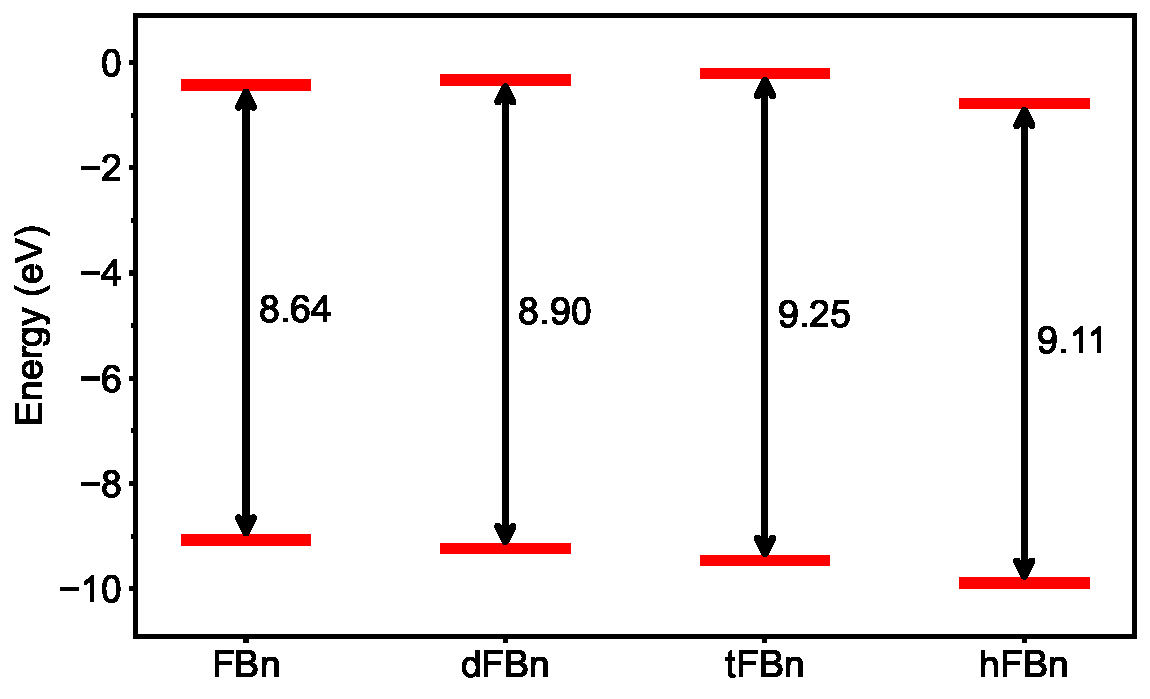
\includegraphics[width=0.7\textwidth]{../figures/data_visualization/HOMO_LUMO_visualization.pdf}
    \caption{HOMO energies, LUMO energies and HOMO-LUMO gap of FBn, dFBn, tFBn and hFBn.}
    \label{fig:4}
\end{figure}

The RF importance analysis (Figure~\ref{Fig.5}A) indicates that HOMO and LUMO energies are the most influential features, with importance scores substantially higher than other molecular descriptors. The HOMO-LUMO gap, dielectric constant, and molecular weight demonstrate moderate importance, while viscosity coefficient and dipole moment contribute relatively little to the model. These results suggest that electronic structure properties play a dominant role in determining ionic conductivity enhancement. The importance of frontier orbital energies is particularly useful: these quantum mechanical descriptors capture the electronic structure of the diluent molecules and reflect their propensity to participate in charge-transfer interactions or coordinate with Li$^+$. A diluent with appropriate HOMO and LUMO energies will exhibit weak donor-acceptor interactions with Li$^+$, minimizing coordination while maintaining sufficient polarity for miscibility\cite{ref.11}.

The permutation importance analysis (Figure~\ref{Fig.5}B) corroborates the overall ranking, with HOMO and LUMO energies emerging as the most important features, followed by dielectric constant and molecular weight. However, several features exhibit relatively large error bars in their importance estimates. This variability can be attributed to correlations between features and the limited size of the dataset. When features are partially redundant, as is often the case with related electronic properties, permuting one feature may not significantly degrade model performance if other correlated features can compensate for the information loss. This leads to instability in importance estimates across different permutation trials. The small number of samples (four diluents) further amplifies these fluctuations, as each permutation represents a substantial perturbation to the limited training data. Despite these limitations, the permutation importance analysis provides a valuable orthogonal perspective that confirms the key role of electronic properties.

\begin{figure}[b]
    \centering
    \begin{subfigure}{0.49\textwidth}
        \begin{overpic}[width=\linewidth]{../figures/feature_analysis/rf_feature_importance.pdf}
            \put(-1,65){\textbf{(A)}}
        \end{overpic}
    \end{subfigure}
    \begin{subfigure}{0.49\textwidth}
        \begin{overpic}[width=\linewidth]{../figures/feature_analysis/permutation_importance.pdf}
            \put(-1,65){\textbf{(B)}}
        \end{overpic}
    \end{subfigure}
    \caption{(A) RF importance and (B) permutation importance of diluent features to ionic conductivity.}
    \label{Fig.5}
\end{figure}

The SHAP analysis (Figure~\ref{fig:6}) provides clear insights into feature contributions, revealing both the magnitude and directionality of each feature's impact on ionic conductivity. LUMO energy, HOMO energy, and dielectric constant exhibit the strongest influence on model predictions. The SHAP summary plot shows that higher values of LUMO energy and HOMO energy are generally associated with positive contributions to ionic conductivity (red points clustered on the positive SHAP value side), while lower values correlate with negative contributions (blue points on the negative side). This relationship helps explain the mechanism: higher (less negative) HOMO energies indicate weaker electron-donating ability, reducing the tendency of the diluent to coordinate with Li$^+$ cations. Similarly, higher (less negative) LUMO energies suggest lower electron affinity, minimizing interactions with anionic species or solvent molecules. Diluents with these electronic characteristics function more effectively as inert spacers that reduce viscosity without disrupting the essential solvation structure.

Dielectric constant also demonstrates a strong positive influence, with higher dielectric constants contributing favorably to ionic conductivity. This can be explained by electrostatic screening effects: diluents with higher dielectric constants more effectively screen charge-charge interactions between ions, reducing ion pairing and facilitating dissociation of ion aggregates. This increases the concentration of free charge carriers available for conduction. However, an excessively high dielectric constant might indicate strong polarity that could lead to undesired coordination with Li$^+$, suggesting that an optimal intermediate range exists.

Molecular weight shows a moderate negative influence, with larger molecular weights generally correlating with reduced ionic conductivity. This trend likely reflects the association between high molecular weight and increased viscosity or reduced molecular mobility. Larger diluent molecules may be less effective at penetrating and disrupting the dense Li$^+$-solvent coordination network, limiting their ability to enhance ion transport. Additionally, high molecular weight diluents occupy greater volume per molecule, potentially leading to unfavorable changes in the electrolyte microstructure at equivalent volume fractions.

The HOMO-LUMO gap exhibits a modest but noticeable effect, with larger gaps associated with positive contributions to conductivity. A wider HOMO-LUMO gap generally indicates greater chemical stability and lower reactivity, suggesting that chemically inert diluents are preferred. This finding aligns with the design principle that diluents should remain electrochemically and chemically passive, serving solely as viscosity modulators rather than active participants in electrochemical reactions or side reactions that could degrade electrolyte performance.

\begin{figure}[t]
    \centering
    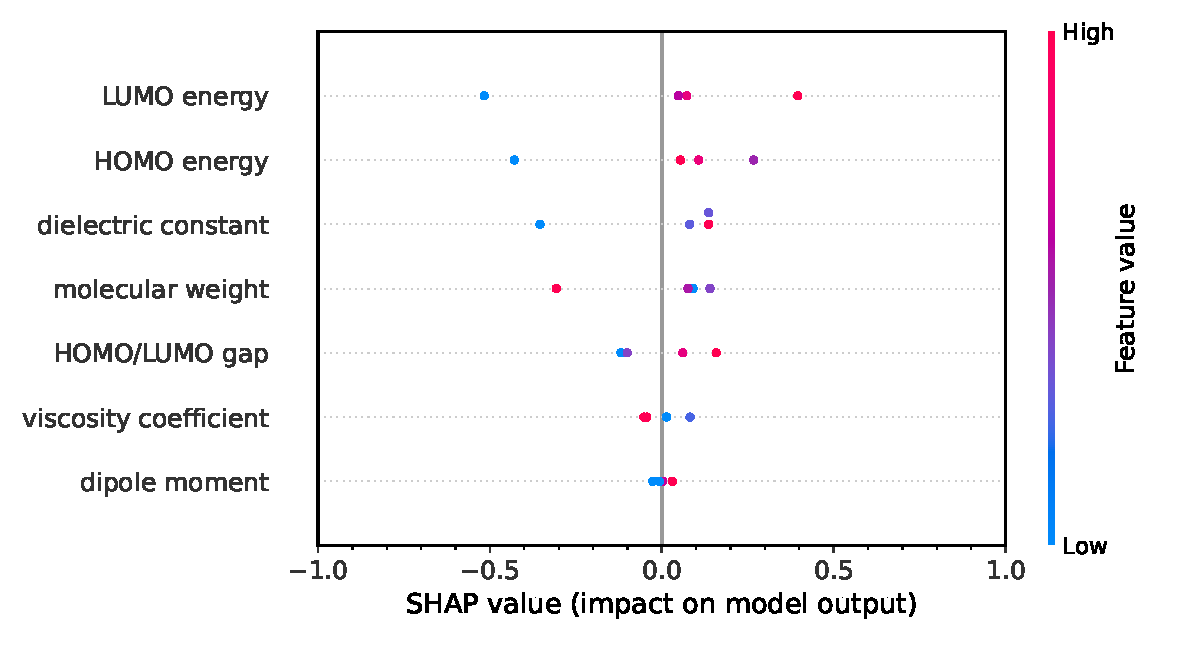
\includegraphics[width=1\textwidth]{../figures/feature_analysis/shap_summary.pdf}
    \caption{SHAP analysis of diluent features to ionic conductivity.}
    \label{fig:6}
\end{figure}

In contrast, viscosity coefficient and dipole moment display SHAP values close to zero, indicating limited direct impact on ionic conductivity within the range of diluents studied. Nevertheless, subtle trends can still be discerned: higher viscosity tends to correlate with slightly negative contributions, as expected from first principles, while larger dipole moments show weak positive correlations. The limited influence of these features is somewhat surprising, given that viscosity directly affects ion mobility and dipole moment reflects polarity. This apparent paradox can be resolved by recognizing that viscosity and polarity are captured indirectly through other features-particularly molecular weight and dielectric constant-that more directly represent the relevant physicochemical properties. Furthermore, the range of viscosity values among the four diluents may not be sufficiently large to manifest a strong correlation in this limited dataset.

The three importance analysis methods yield slightly different feature rankings. These discrepancies arise from differences in their underlying mathematical frameworks. RF importance is based on impurity reduction during decision tree construction and may be biased toward features with high variance or those that facilitate early splits in the tree structure. Permutation importance measures the degradation in model performance when a feature is randomly shuffled, providing a more direct assessment of predictive utility but potentially suffering from instability when features are correlated or datasets are small. SHAP analysis, grounded in cooperative game theory, offers the most rigorous and interpretable framework by computing the marginal contribution of each feature across all possible feature subsets. This approach ensures consistency and fairness in attribution, accounting for feature interactions and providing both global importance rankings and local explanations for individual predictions.

Among these methods, SHAP is generally considered the gold standard for model interpretation due to its theoretical soundness and ability to provide consistent, unbiased feature attributions. Therefore, the SHAP results serve as the primary basis for interpreting feature effects in this study, while the complementary RF and permutation importance analyses provide corroborating evidence and alternative perspectives.

\subsection{Integrating Insights: Toward Rational Diluent Design}

The convergence of evidence from multiple analytical approaches establishes that electronic properties (HOMO and LUMO energies), dielectric constant, and molecular weight are the key determinants of ionic conductivity enhancement in fluorinated benzene diluent systems. These findings suggest design principles for next-generation electrolyte diluents: optimal candidates should possess (1) high HOMO and LUMO energies to minimize unwanted coordination with Li$^+$ and maintain electrochemical inertness, (2) moderate-to-high dielectric constants to facilitate ion dissociation through electrostatic screening, and (3) relatively low molecular weights to maximize molecular mobility and minimize viscosity contributions.

The case of tFBn exemplifies these principles: its three fluorine substituents elevate both HOMO and LUMO energies while maintaining sufficient polarity (intermediate dielectric constant) and relatively low molecular weight. This combination positions tFBn in an optimal region of the molecular descriptor space, explaining its superior performance. Conversely, hFBn's excessive fluorination drives the molecule toward extremely high frontier orbital energies and very low polarity, causing poor miscibility and inadequate screening effects despite its low coordination tendency. FBn and dFBn, with insufficient fluorination, retain partial coordination character and fail to achieve the requisite balance of properties.

This structure-property understanding provides guidance for future electrolyte design. By computationally screening candidate diluents and tuning molecular features through systematic variation of fluorination patterns, functional group substitutions, or structural scaffolds within the optimal ranges identified here, it becomes possible to design diluents that maximize ionic conductivity while preserving electrochemical stability. Beyond the specific case of fluorinated benzene derivatives, the analytical framework demonstrated in this study offers a generalizable strategy for accelerating materials discovery: coupling experimental measurements with machine learning-based feature analysis to extract interpretable design rules from limited datasets.

Moreover, this work reflects a growing trend of AI-assisted materials science, in which data-driven methods augment traditional chemical intuition to uncover hidden structure-property relationships and guide the development of advanced functional materials. As experimental and computational datasets continue to grow, such approaches may help accelerate the optimization of complex systems like electrolytes, catalysts, and functional polymers, helping improve future research of rational materials design.

\clearpage

\section{Conclusion}

This study presents a data-driven approach for the rational design of high-conductivity electrolytes, demonstrating how the strategic integration of experimental measurements, quantum chemical calculations, and machine learning can be used to derive design principles from limited data. By investigating fluorinated benzene diluents in localized high-concentration electrolyte systems, the fundamental structure-property relationships that govern ionic conductivity enhancement are uncovered and a methodological template applicable to diverse materials challenges in energy storage has been established.

This study has three main findings. First, it reveals that the non-monotonic conductivity behavior reflects an intrinsic competition between viscosity reduction at low diluent concentrations and ion dilution at high concentrations—a mechanistic insight that provides clear boundaries for optimal electrolyte formulation. Second, through systematic model comparison, this study demonstrates that predictive accuracy depends not on algorithmic complexity but on matching model sophistication to dataset characteristics, with a third-order polynomial outperforming advanced machine learning methods in our constrained data regime. This finding provides guidance for the many materials science problems where data scarcity is the norm rather than the exception. Third, this study employs Shapley additive explanations to systematically dissect the contributions of seven molecular features, identifying frontier orbital energies and dielectric constant as the dominant factors controlling conductivity. This mechanistic understanding enables a transition from empirical optimization to rational molecular design.

These results may also be applied beyond the specific fluorinated diluent systems studied here. By demonstrating that interpretable machine learning can extract predictive design rules from minimal experimental data, a possible approach for materials discovery across energy storage, catalysis, and functional materials is established. This approach helps address a common challenge in materials science: most problems lack the large datasets required for conventional machine learning, yet still demand rapid optimization. The framework constructed in this paper shows that even with four diluents, rigorous feature analysis can identify the critical molecular descriptors and establish design principles with predictive power.

This work reflects a growing trend of AI-assisted materials science, where computational tools augment rather than replace experimental insight. The integration of quantum chemical calculations with experimental measurements and machine learning creates a virtuous cycle: calculations provide molecular descriptors, experiments validate predictions, and machine learning identifies patterns that guide the next iteration of design. This hybrid approach improves research efficiency and helps deepen mechanistic understanding by forcing explicit consideration of which molecular features truly matter.

Looking forward, the strategies developed here are directly applicable to pressing challenges in next-generation battery development, including the design of solid-state electrolytes, the optimization of electrode-electrolyte interfaces, and the development of electrolytes for emerging chemistries such as lithium-sulfur and lithium-air systems. In addition, as artificial intelligence becomes increasingly central to scientific discovery, frameworks that maintain interpretability while leveraging computational power (as demonstrated here) will prove essential for accelerating innovation while preserving the mechanistic insight that enables true understanding.

In summary, this work provides a useful method that demonstrates how data-driven approaches can be rigorously applied to small-data problems in materials science, yielding both immediate practical guidance for electrolyte optimization and a generalizable template for AI-assisted materials design. As the energy research community confronts the urgent need to accelerate the development of sustainable technologies, such integrative frameworks offer a possible path toward improving materials discovery from a largely empirical endeavor into a rational, predictive discipline.

% --- AI Process Disclosure (required by AIDER) ---
\section*{AI Process Disclosure}

This research was conducted with AI assistance. The complete process log,
including all AI agent transcripts, prompts, and a timestamped record of
human decisions, is available in the
\href{\repourl/tree/main/process-log}{process-log directory} of the
paper repository.

% Tools used, scope of AI involvement, and human oversight should be
% summarised here. Full details belong in the process-log/ directory.

% --- Acknowledgements ---
\section*{Acknowledgements}

This work was financially supported by the JST SPRING (Grant NO. JPMJSP2110).

% --- References ---

\printbibliography[title={References}]

\end{document}
